\chapter{Experiments and Evaluations}
\label{ch:experiments}

This chapter presents details of the experiments and evaluations for the proposed test scripts in the previous chapter.
First, we describe the environment setup for testing process.
Subsequently, we present all the experiments along with evaluation and assessment for each of them.

\section{Experimental environment}

\subsection{Hardware configurations}
All test suites are conducted with the hardware configurations as shown in table \ref{tab:hw}. We use 2 phones running 2 different \acrshort{os} versions with different screen size and resolution for testing the portability of the system.

\begin{table}[H]
	\centering
	\caption{Hardware configuration for testing process}	
	\label{tab:hw}
	\begin{tabularx}{0.65\textwidth}{ll}
		\toprule
		Phone 1 & ASUS Zenfone 5 \\
			  & Resolution 720 x 1280 pixels \\
			  & Screen 5'' 6.22 cm x 11.06 cm \\
			  & Android 5.0.1\\
		\midrule 
		Phone 2 & Sony XPeria L \\
			  & Resolution 480 x 850 pixels \\
			  & Screen 4.3'' 5.40 cm x 9.60 cm \\
			  & Android 4.2.2\\
		\midrule 
		Robot & Self-construct Delta Robot with stylus \\
			  & \begin{minipage}{0.7\linewidth}
			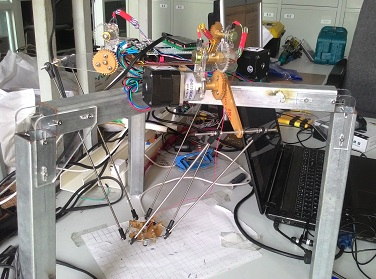
\includegraphics[width=0.8\linewidth]{Chapters/Fig/delta_robot.jpg}
		\end{minipage} \\
		\midrule 
		Computer & Windows \acrshort{pc} \\
				 & Having 2 \acrshort{usb} ports for connecting the phone and the robot. \\
		\bottomrule
	\end{tabularx}
\end{table}

\subsection{Supporting software}
The application can not operate lonely. It requires some supporting software on the computer and applications to be tested installed on target phones.

	\begin{itemize}
		\item[--] \textbf{Android platform tool}: command line tools for communicate with Android device.
		\item[--] \textbf{Droid@Screen}: application letting us capture Android screen to acrshort{pc}.
		\item[--] \textbf{Simple Click Test} \footnote{Source code available at: \url{https://github.com/alfrededison/simple-click-test}}: self-created tested application for Experiment 1.
		\item[--] \textbf{Clock ICS} \footnote{Download available at Google Play Store: \url{https://play.google.com/store/apps/details?id=com.moblynx.clockics}}: tested application for Experiment 2.
	\end{itemize}

\subsection{Experimental procedure}
First, set the phone to the calibrated position of the robot's pointer.

	\begin{figure}[H]
		\centering
		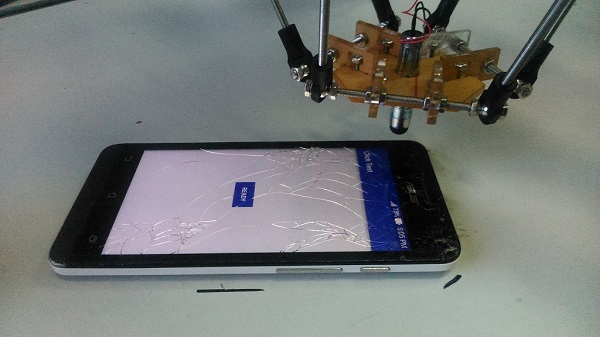
\includegraphics[scale=0.5]{Chapters/Fig/phone_setup.jpg}
		\caption{Setup phone position}
		\label{fig:phone_setup}
	\end{figure}

Then open Droid@Screen application to capture phone screen. See Appendix \ref{ch:img_capture} for capturing process's detail.

	\begin{figure}[H]
		\centering
		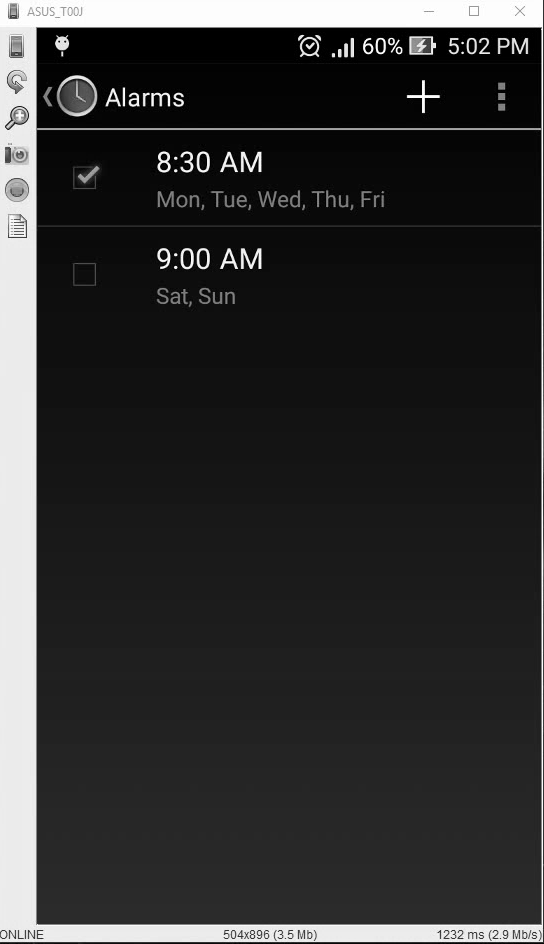
\includegraphics[scale=0.5]{Chapters/Fig/droidscreen.png}
		\caption{Capture phone screen}
		\label{fig:droidscreen}
	\end{figure}

Finally, open the program and set up the parameters

	\begin{figure}[H]
		\centering
		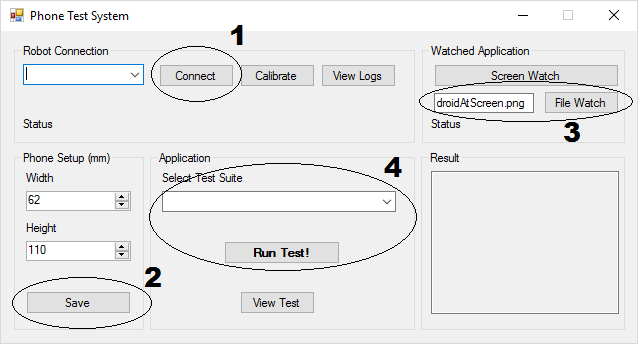
\includegraphics[scale=0.5]{Chapters/Fig/prog_setup.png}
		\caption{Parameter setup}
		\label{fig:prog_setup}
	\end{figure}

	\begin{itemize}
		\item[--] Connect to the robot by choosing COM port and press Connect.
		\item[--] Configure phone size
		\item[--] Choose screen watching method
		\item[--] Select test suite and run the test
	\end{itemize}

\section{Experiments and Results}
This section gives the details of all experiments that we have conducted to verify and evaluate the accuracy of Delta robot as well as the whole Testing System proposed in the previous chapter.

\subsection{Experiment 1: Test robot accuracy}
\subsubsection{Experimental purpose}
By letting the Delta robot move around the phone screen, we can test the working accuracy of the robot under certain repeated actions.

\subsubsection{Experimental setup}
	\begin{itemize}
		\item[--]Open Click test application on the phone. Let the application be at initial page.
		\item[--]Follow the experimental procedure mentioned in previous section.
	\end{itemize}

\subsubsection{Experimental results}
Begin test screen, the robot need to click on READY button.
	\begin{figure}[H]
		\centering
		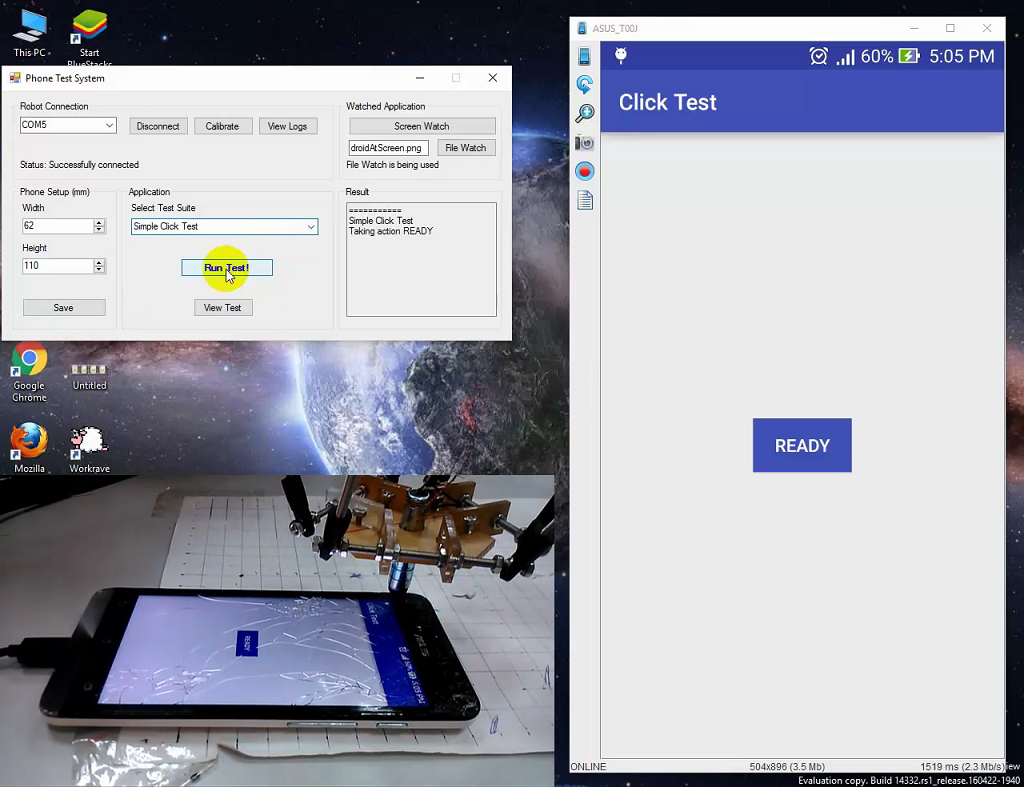
\includegraphics[scale=0.5]{Chapters/Fig/click_start.png}
		\caption{Begin click test screen}
		\label{fig:click_start}
	\end{figure}

After clicking on READY, SUCCESS button appears. The robot is commanded to click on it.

	\begin{figure}[H]
		\centering
		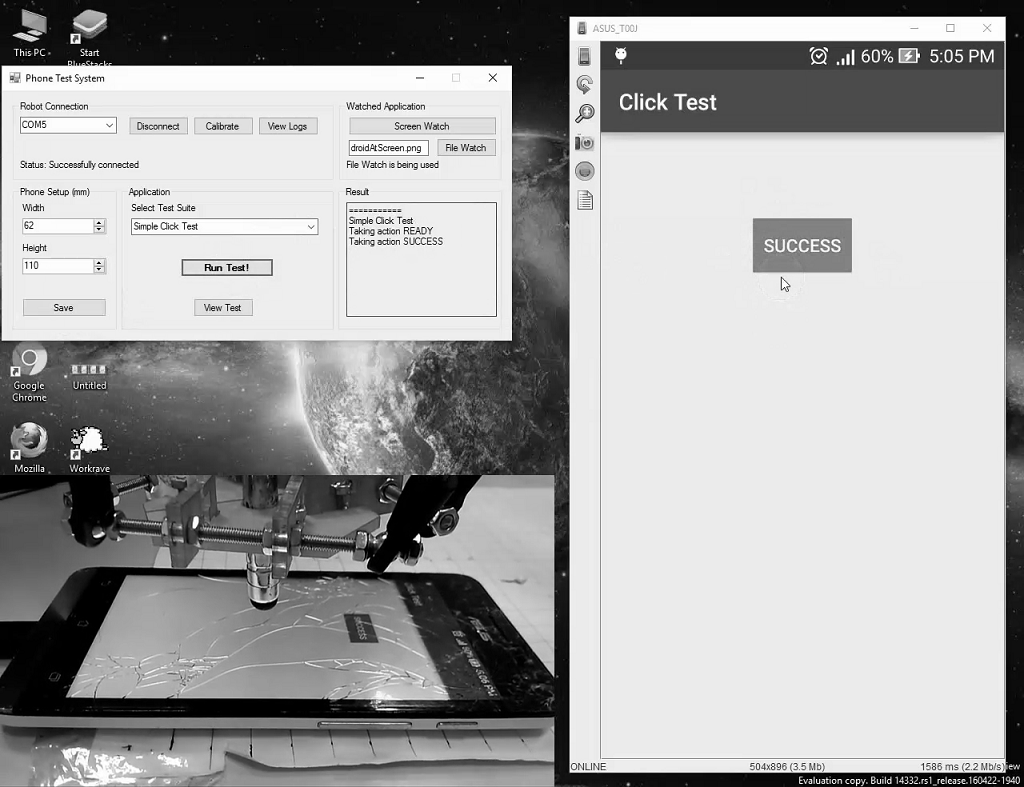
\includegraphics[scale=0.5]{Chapters/Fig/click_mid.png}
		\caption{After clicking READY screen}
		\label{fig:click_mid}
	\end{figure}

Final result when READY is clicked. The test is Passed.
	\begin{figure}[H]
		\centering
		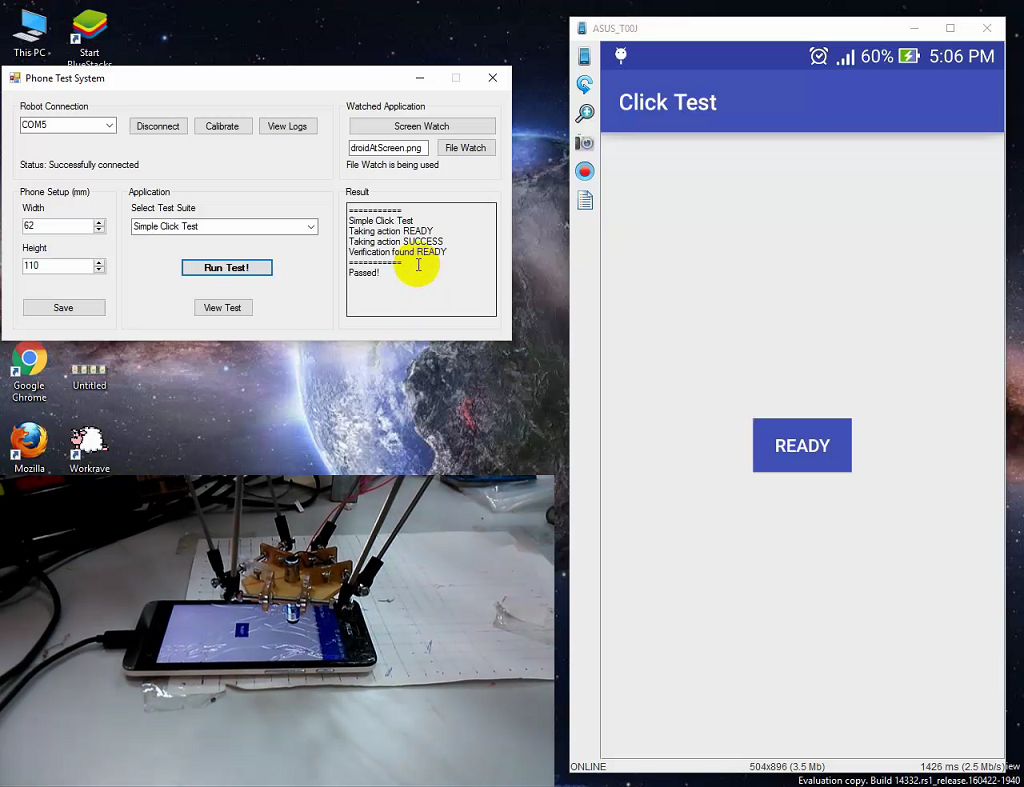
\includegraphics[scale=0.5]{Chapters/Fig/click_final.png}
		\caption{Final click test screen}
		\label{fig:click_final}
	\end{figure}

\subsection{Experiment 2: Set alarm time}
\subsubsection{Experimental purpose}
This experiment is conducted to verify the smooth in movement of the robot while dragging an item on the phone screen as well as the precision in clicking items.

In addition, this test can be considered as a real test case for an alarm application on Android phones that the tester has to carry out before releasing the application to the market.

\subsubsection{Experimental setup}
	\begin{itemize}
		\item[--]Open Clock ICS application on the phone. Switch to Alarms screen of the application.
		\item[--]Follow the experimental procedure in previous section.
	\end{itemize}

\subsubsection{Experimental results}
Before running the test, initial alarms are 8:30 AM and 9:00 AM. The goal of the test is to change 8:30 AM to 11:30 AM.

	\begin{figure}[H]
		\centering
		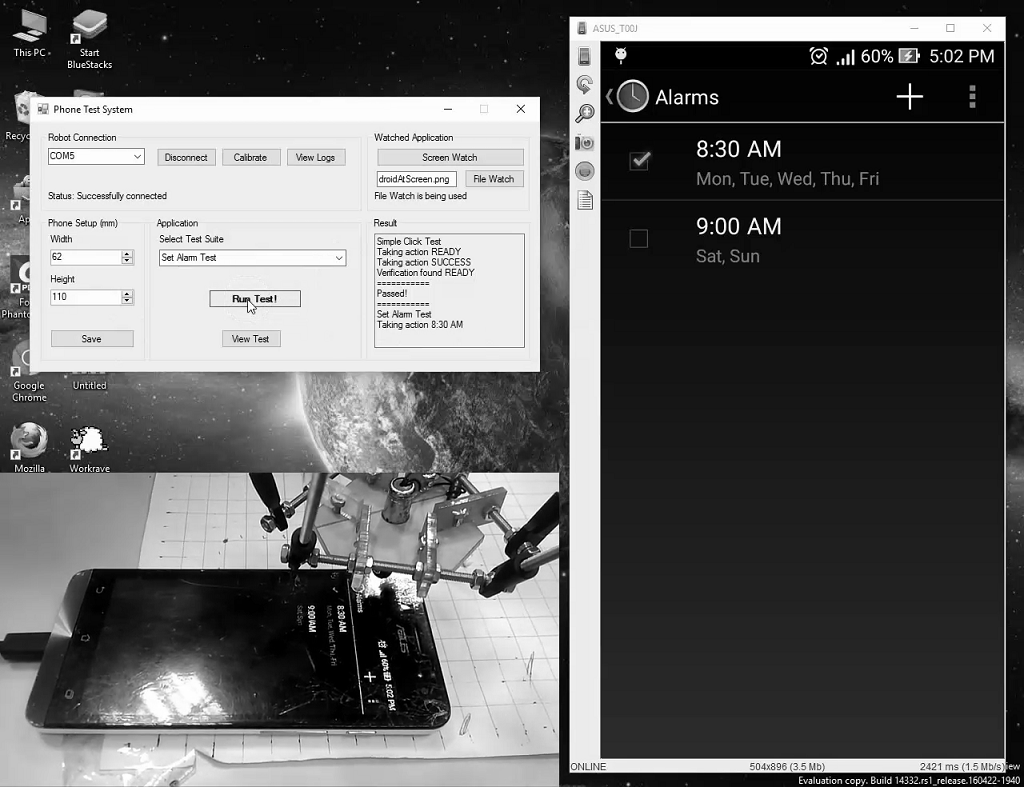
\includegraphics[scale=0.5]{Chapters/Fig/alarm_start.png}
		\caption{Begin alarm test}
		\label{fig:alarm_start}
	\end{figure}

After proceeding some operations, the final screen of the application is shown below. 11:30 AM shows up and the test is successfully passed.

	\begin{figure}[H]
		\centering
		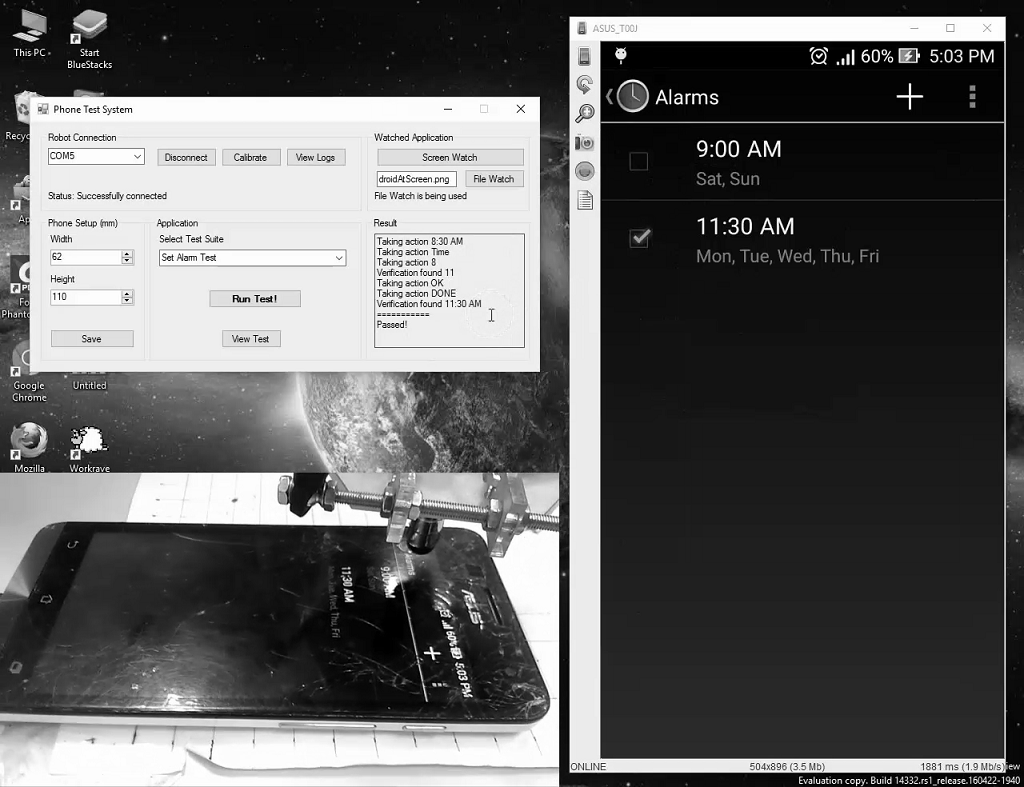
\includegraphics[scale=0.5]{Chapters/Fig/alarm_final.png}
		\caption{Final alarm test}
		\label{fig:alarm_final}
	\end{figure}

\subsection{Experiment 3: Set alarm label}
\subsubsection{Experimental purpose}
This experiment is conducted to verify the high-demanded precision in clicking items.

In addition, this test can also be considered as a real test case for an alarm application on Android phones that the tester has to carry out before releasing the application to the market.

\subsubsection{Experimental setup}
Set up as Experiment 2.

\subsubsection{Experimental results}
Before running the test, initial alarms are 8:30 AM with no label.

	\begin{figure}[H]
		\centering
		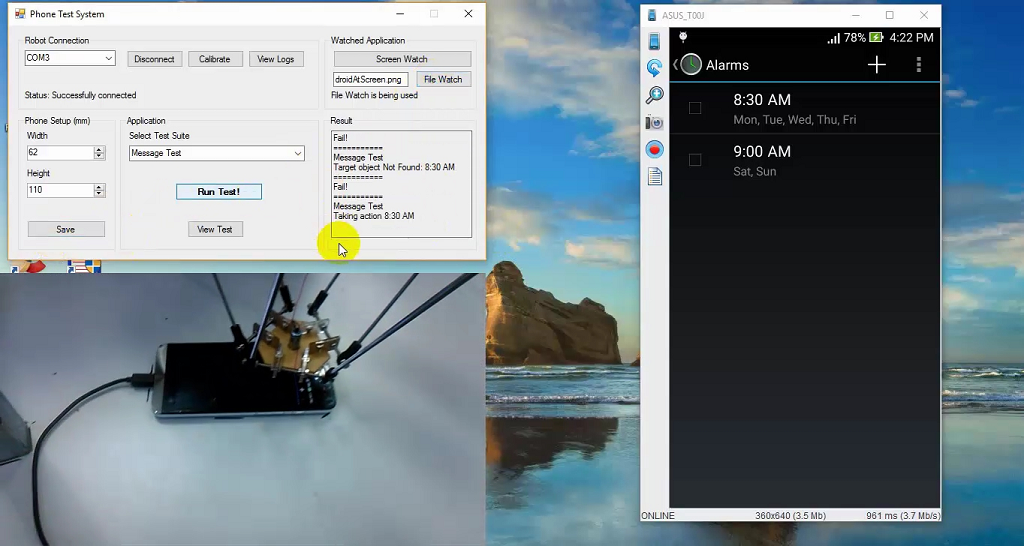
\includegraphics[scale=0.5]{Chapters/Fig/label_first.png}
		\caption{Begin typing test}
		\label{fig:label_first}
	\end{figure}

After proceeding some operations, the final screen of the application is shown below. 8:30 AM has label ``i love DCE'' on the right. The test is successfully passed.

	\begin{figure}[H]
		\centering
		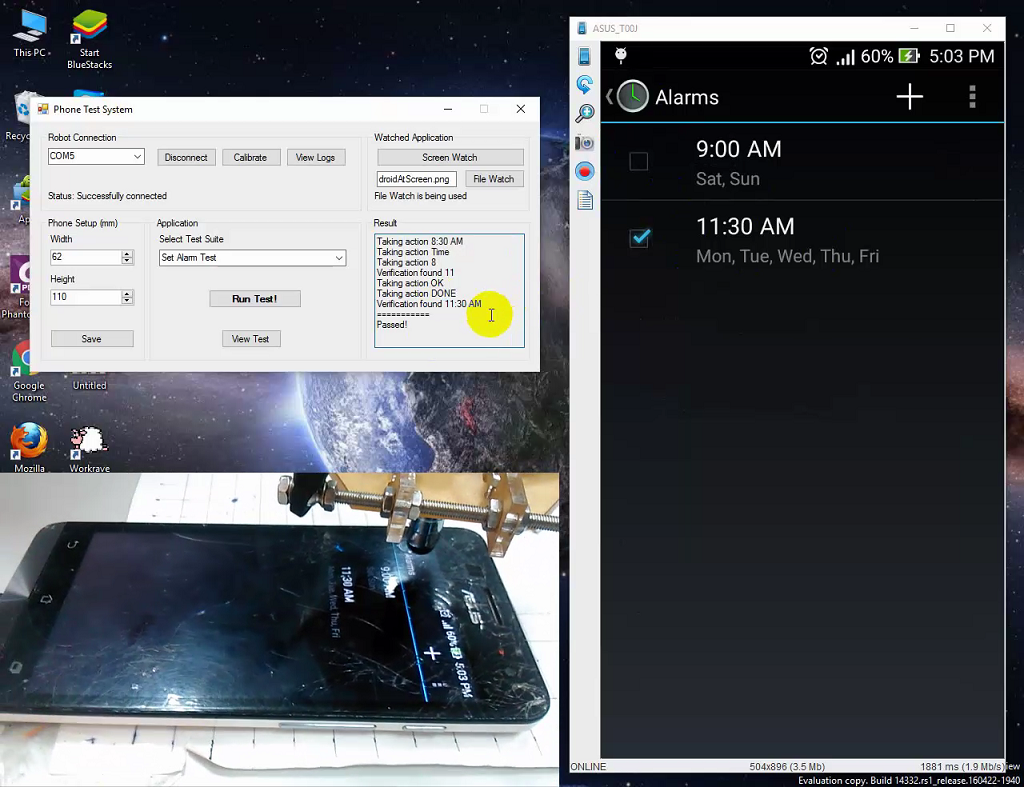
\includegraphics[scale=0.5]{Chapters/Fig/label_final.png}
		\caption{Final typing test}
		\label{fig:label_final}
	\end{figure}

\section{Analysis and evaluation}
By conducting all the tests over and over, we attain an overview about the reliability, usability and durability of the system.

\subsection{Results statistics and analysis}
All the test results are recorded in Table \ref{tab:result_stat}. In general, the system produces a high production rate.

	\begin{table}[H]
		\centering
		\caption{Test results statistic}	
		\label{tab:result_stat}
		\begin{tabular}{|l|rrr|}
			\hline
			Test case & Successful & Failed & Number of tests \\
			\hline
			Simple Click & 10 & 0 & 10 \\
			Set Alarm & 5 & 5 & 10 \\
			Typing & 3 & 7 & 10 \\
			\hline
			Total & 18 & 12 & 30 \\
			\hline
			\textbf{Rate} & \textbf{0.6} & \textbf{0.4} & \textbf{1.00} \\
			\hline
		\end{tabular}
	\end{table}

For simple application such as Simple Click, the system reaches absolute preciseness thus not any problem is made.

Alarm Test, however, is more complicated and requires much more conditions. With high definition display, Zenfone 5 gives us completely successful results. In contrast, XPeria L has lower resolution screen that makes some obstacles in \acrshort{ocr}. Therefore, a bad result is returned.

Typing Test is more and more complicated. It requires the best movements of the robot. Furthermore, the screen size has to be large enough for the stylus to click on the correct keys. The result is not very good due to the limitation of stylus size and screen size.

\subsection{Evaluation}
\subsubsection{Reliability}
Due to the fact that current \acrshort{ocr} engine has limitation in recognizing character in low resolution, the system makes some false negative errors. This demands us to equip a better recognition module in later research.

\subsubsection{Usability}
With good image quality, instead, the system performs every action precisely with no such an error. With the ease of use and few actions required, we believe that the system is suitable for all test in the industry.

\subsubsection{Durability}
The robot can perform one action over high intensity of repetition without any mistake. This advantage helps the system to hold a high stability over time.
